\section{Mạng Ethereum}

\subsection{Lịch sử}

Ethereum là một nền tảng mã nguồn mở dựa trên chuỗi khối, hỗ trợ \textit{Hợp đồng thông minh}\footnote{Smart contract}. Ethereum khá nổi với \textit{đồng tiền mã hoá}\footnote{Cryptocurrency} của nó với tên gọi là \textit{Ether} (ký hiệu: ETH). Dựa vào sự phân tán của công nghệ chuỗi khối, Ethereum khá an toàn, và cũng nhờ bảo mật cao nên giá trị của đồng tiền ETH tích luỹ ngày càng lớn trên thị trường tiện điện tử.\\

Bắt đầu ý tưởng từ năm 2013 bởi lập trình viên \href{https://en.wikipedia.org/wiki/Vitalik_Buterin}{\textit{Vitalik Buterin}} và một số cộng sự, công việc phát triển Ethereum được vận hành và kêu gọi vốn từ cộng đồng vào năm sau đó. Mạng Ethereum chính thức "lên sóng" vào ngày 30 tháng 7 năm 2015.\\

\subsection{Hợp đồng thông minh}

Nền tảng Ethereum còn hỗ trợ mạng lưới các \textit{ứng dụng phi tập trung}\footnote{Decentralized applications (DApps)}. Mạng này vận hành xoay quanh các hợp đồng thông minh. Phần lớn các ứng dụng sử dụng hợp đồng thông minh để liên kết với công nghệ chuỗi khối. Có thể nói, hợp đồng thông minh chính là nhân tố trung tâm của nền tảng Ethereum.\\

Hợp đồng thông minh là \textit{hợp đồng tự thực thi}\footnote{Self-executed contract} với các điều khoản được viết bởi các dòng lệnh hay các đoạn mã lập trình. Các đoạn mã này tồn tại khắp các nút trong mạng chuỗi khối, điều hành sự thực thi các giao dịch, và không thể thay đổi. Hợp đồng thông minh mang đến các giao dịch đáng tin cậy, sự đồng ý với các điều khoản trong hợp đồng tới các bên "ẩn danh" mà không cần qua một bên trung gian hay một cơ chế thực thi bên ngoài.\\

Trên Ethereum, các đoạn mã của hợp đồng thông minh được viết bằng ngôn ngữ lập trình \textit{Solidity} hoặc \textit{Vyper}. Solidity là ngôn ngữ lập trình hướng đối tượng bậc cao dựa theo \textit{C++}, \textit{JavaScript}, \textit{Python}, và được thiết kế để tích hợp được với \textit{Máy ảo Ethereum}\footnote{Ethereum Virtual Machine - EVM} (EVM). Vyper là ngôn ngữ đang trong quá trình thử nghiệm.\\

\subsection{Chi phí giao dịch}

\textit{Gas} là đơn vị thể hiện cho khối lượng tính toán để thực hiện một hành động nào đó trên mạng Ethereum. Do mỗi giao dịch trên mạng Ethereum đều cần tài nguyên tính toán để được thực thi, vì thế mà nó phát sinh ra \textit{chi phí giao dịch}. Khi đó, \textit{gas} thể hiện chi phí để thực hiện giao dịch thành công trên mạng.\\

\begin{figure}[ht]
    \centering
    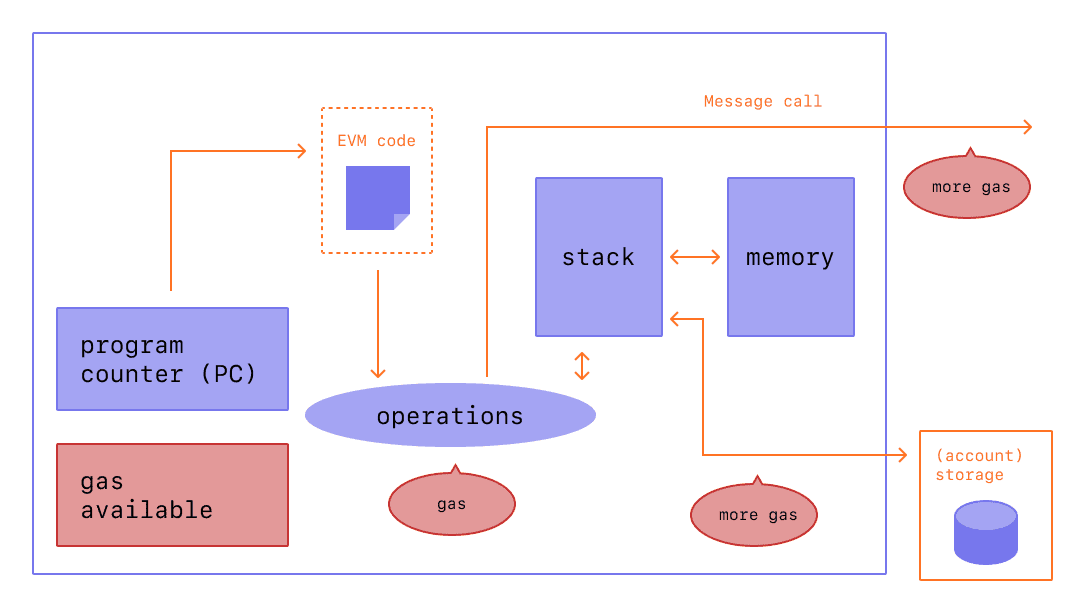
\includegraphics[width=400px]{images/gas.png}
\end{figure}

\textit{Gas} được trả bằng đồng \textit{ether} (ETH). \textit{Giá gas}\footnote{Gas price} có đơn vị là \textit{gwei}, mỗi \textit{gwei} tương ứng với một phần một tỷ của một \textit{ether}: $1$ \textit{gwei} $=10^{-9}$ \textit{ether}. Vì vậy, thay vì nói chi phí giao dịch là $0,000000001$ \textit{ether}, ta có thể nói giao dịch đó tiêu tốn $1$ \textit{gwei}. Ngoài ra, $1$ \textit{gwei} chính là một tỷ \textit{wei}; \textit{wei} (được đặt tên theo \textit{Wei Dai} - nhà khoa học máy tính nổi tiếng đưa ra lý thuyết về thanh toán bằng tiền mã hoá) là đơn vị nhỏ nhất trên Ethereum.\\

